\documentclass[aspectratio=169]{beamer} % dvipsnames gives more built-in colors

\usepackage{}
\usepackage{bibentry}
\usepackage{scalefnt}
\usepackage{graphicx}
\usepackage{epstopdf}
% \usepackage{multimedia}
\usepackage{media9}

% \epstopdfDeclareGraphicsRule{.gif}{png}{.png}{convert gif:#1 png:\OutputFile}
% \AppendGraphicsExtensions{.gif}

\usetheme{Madrid}
\useoutertheme{miniframes} % Alternatively: miniframes, infolines, split
\useinnertheme{circles}

\definecolor{UBCblue}{rgb}{0.04706, 0.13725, 0.26667} % UBC Blue (primary)

\usecolortheme[named=UBCblue]{structure}
% \usecolortheme[named=Mahogany]{structure} % Sample dvipsnames color

\title[DP in semantic segmentation]{A survey on deep learning techniques in image and video semantic segmentation}
\subtitle{(paper analysis)}
\date{June, 2020}

\author[J\'{e}ssica Motta]{J\'{e}ssica Motta}
\institute[SENAI CIMATEC]{SENAI CIMATEC}
\titlegraphic{\begin{flushright}
  
\includegraphics[width=2cm]{Template/logosenaicimatec}
\end{flushright} 
}

\graphicspath{{Media/pictures/}}

\begin{document}

\begin{frame}
  \titlepage
\end{frame}

%*----------- SLIDE -------------------------------------------------------------
\begin{frame}[t]{Concept Map} 
    \begin{figure}
        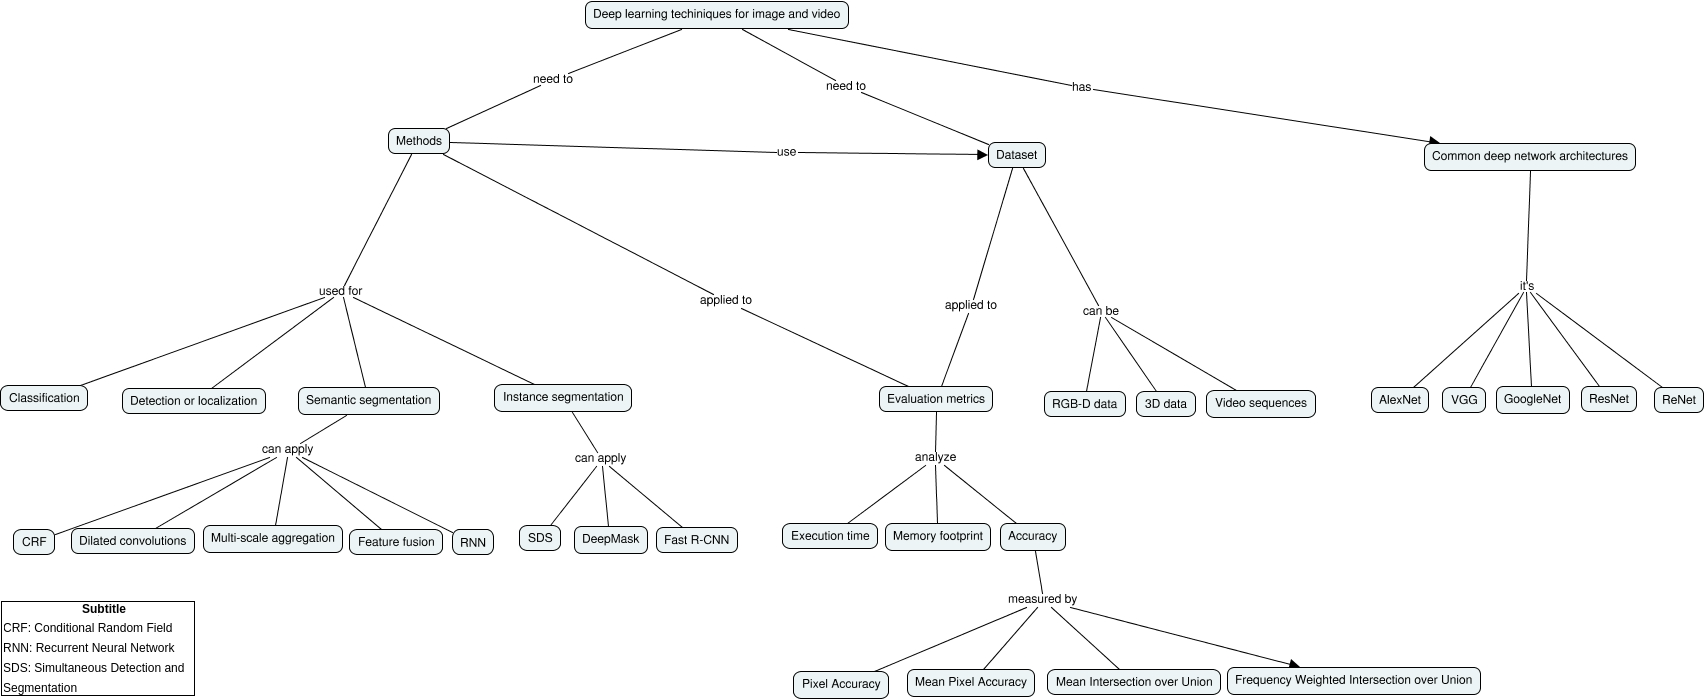
\includegraphics[width=0.95\textwidth]{concept_map_paper2_jess}
        \caption{Fonte: Own authorship.}
    \end{figure}
\end{frame}


%*----------- SLIDE -------------------------------------------------------------
\begin{frame}[t]{CNN- How it works?}
    \begin{figure}[h]
        
        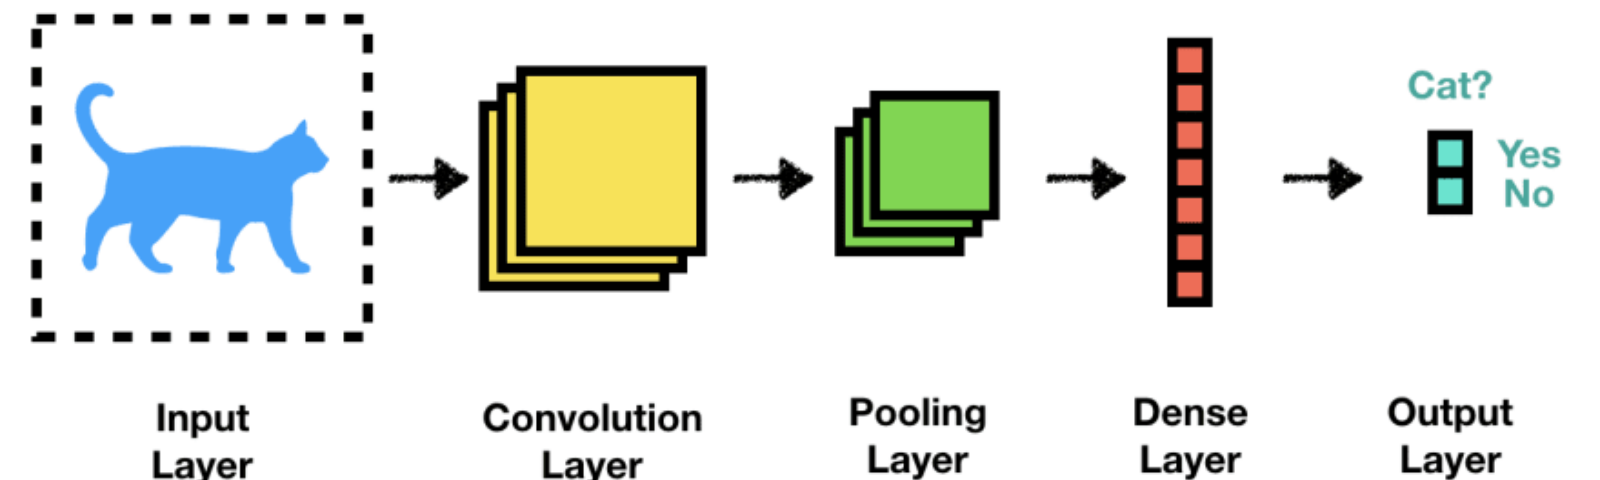
\includegraphics[width=0.90\textwidth]{cnn}
        \caption{Convolutional Neural Network \cite{CNN}}   
    \end{figure}
\end{frame}
%*----------- SLIDE -------------------------------------------------------------
\begin{frame}[t]{Common deep networks architecture}
    \vspace{0.5cm}
    \begin{table}[]
        \begin{tabular}{|c|c|c|c|}
        \hline
        \multicolumn{4}{|c|}{\textbf{COMPARATIVE FOR COMMON DEEP NETWORK ARCHITECTURES}}                 \\ \hline
        \textbf{Network} & \textbf{Year champion ILSVRC*} & \textbf{Number of Layers} & \textbf{Accuracy} \\ \hline
        AlexNet          & 2012                          & 3                         & 84.6\%            \\ \hline
        VGG              & 2013                          & 16                        & 92.7\%            \\ \hline
        GoogleNet        & 2014                          & 22                        & 93.3\%            \\ \hline
        ResNet           & 2016                          & 152                       & 96.4\%            \\ \hline
        \end{tabular}
        \caption{Deep network architectures. \cite{garcia2018survey}}
        \label{tab:deep-net}
        \end{table}

    *ILSVRC (ImageNet Large Scale Visual Recognition Challenge)
   
\end{frame}
%-

%*----------- SLIDE -------------------------------------------------------------
\begin{frame}[t]{Methods to image analysis} %pensar no que colocar
    \begin{figure}
        \centering
        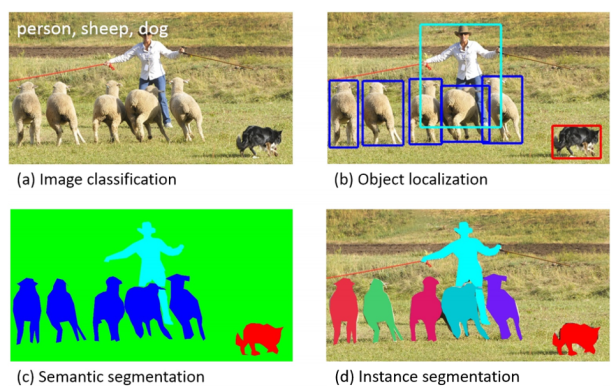
\includegraphics[width=0.55\textwidth]{methods}
        \caption{Methods to image analysis. \cite{lin2014microsoft}}
    \end{figure}
\end{frame}
%-

%*----------- SLIDE -------------------------------------------------------------
\begin{frame}[t]{Evaluation Metrics} %pensar no que colocar
    \begin{columns}[c]
        \column{.05\textwidth}
        \column{.6\textwidth}
            \newline
            \newline
                Execution time
            \newline
            \newline
                Memory footprint
            \newline
            \newline
                Accuracy
           
        \column{.35\textwidth}
            
\includegraphics[width=0.5\textwidth]{accuracy}\hspace*{6cm}
            
    \end{columns}


\end{frame}
%-

%*----------- SLIDE -------------------------------------------------------------
\begin{frame}[t]{Accuracy} %pensar no que colocar
    \begin{figure}
        \centering
        
       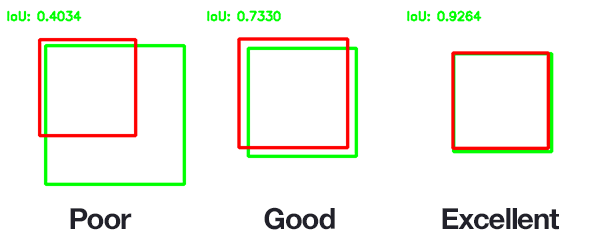
\includegraphics[width=0.6\textwidth]{iou}
       \caption{Accuracy evaluation. \cite{IoU}}
    \end{figure}
\end{frame}
%-
% %*----------- SLIDE -------------------------------------------------------------
% \begin{frame}[t]{Accuracy results } %pensar no que colocar
%         \begin{table}[]
%                 \scalefont{0.55}
%                 \begin{tabular}{|c|c|c|c|c|c|c|c|c|c|}
%                 \hline
%                 \multicolumn{10}{|c|}{\textbf{ACCURACY RESULTS (METHODS AND DATASETS) (\%)}}     \\ \hline
%                 \textbf{Method / Dataset} &
%                   \textbf{\begin{tabular}[c]{@{}c@{}}PASCAL \\ VOC-2012\end{tabular}} &
%                   \textbf{\begin{tabular}[c]{@{}c@{}}Pascal- Person- \\ Part\end{tabular}} &
%                   \textbf{CamVid} &
%                   \textbf{CityScapes} &
%                   \textbf{\begin{tabular}[c]{@{}c@{}}Stanford \\ Background\end{tabular}} &
%                   \textbf{SiftFlow} &
%                   \textbf{SUN3D} &
%                   \textbf{\begin{tabular}[c]{@{}c@{}}ShapeNet \\ Part\end{tabular}} &
%                   \textbf{\begin{tabular}[c]{@{}c@{}}Youtube- \\ Objects\end{tabular}} \\ \hline
%                 \textbf{PSPNet}            & 85,4 &       &       &       &       &  &       &       &       \\ \hline
%                 \textbf{DeepLab}           &      & 64,94 &       &       &       &  &       &       &       \\ \hline
%                 \textbf{DAG-RNN}           &      &       & 91,60 &       &       &  &       &       &       \\ \hline
%                 \textbf{rCNN}              &      &       &       &       & 80,20 &  &       &       &       \\ \hline
%                 \textbf{LSTM-CF}           &      &       &       &       &       &  & 58,50 &       &       \\ \hline
%                 \textbf{PointNet}          &      &       &       &       &       &  &       & 83,70 &       \\ \hline
%                 \textbf{PointNet++}        &      &       &       &       &       &  &       & 85,10 &       \\ \hline
%                 \textbf{DGCNN}             &      &       &       &       &       &  &       & 85,10 &       \\ \hline
%                 \textbf{Clockwork Convent} &      &       &       &       &       &  &       &       & 68,50 \\ \hline
%                 \textbf{SegmPred}          &      &       &       & 59,40 &       &  &       &       &       \\ \hline
%                 \end{tabular}
%                 \caption{Accuracy results for the most relevant methods and dataset. \cite{garcia2018survey}}
%                 \label{tab:accuracy_results}
%                 \end{table}
% \end{frame}

%*----------- SLIDE -------------------------------------------------------------
\begin{frame}[t]{Wich cases doesn't apply deep learning?} %usar limitations?
        \begin{columns}[c]
                \column{.05\textwidth}
                \column{.6\textwidth}
                        For \textbf{high perfomance}, deep networks require \textbf{extremely large} datasets.  
                        \newline
                        \newline
                        It's \textbf{expensive} to get data, computer power and hiring researchers.
                        \newline
                        \newline
                        Deep networks \textbf{aren't easily interpreted} as classical Machine Learning algorithms.
                \column{.35\textwidth}
                    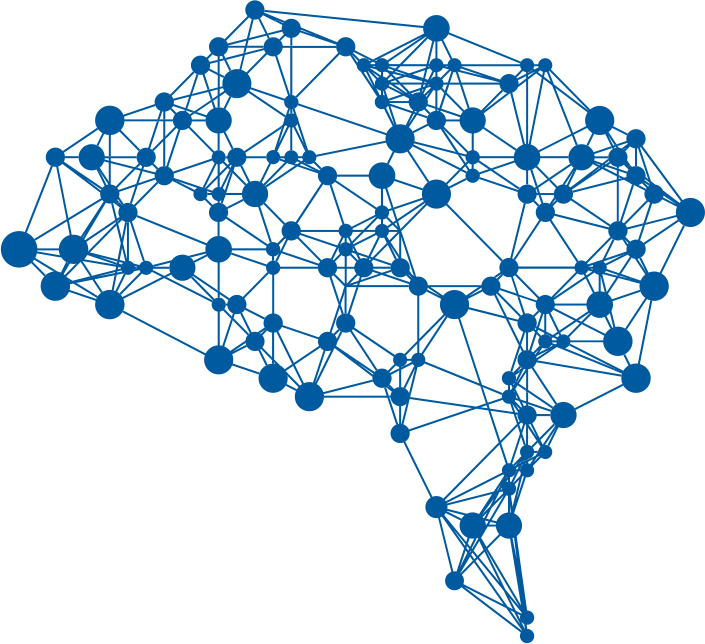
\includegraphics[width=0.9\textwidth]{dnn}
            \end{columns}
        
    
\end{frame}
%-

%*----------- SLIDE -------------------------------------------------------------
\begin{frame}[t]{Advantages to use Deep learning against to Classical methods} 
        \begin{columns}[c]
                \column{.05\textwidth}
                \column{.6\textwidth}
                \newline
                \newline
                \textbf{Better} performance (accuracy results)
                \newline
                \newline
                More data works to DP \textbf{but not} with CML
                \newline
                \newline
                DP \textbf{no need} for feature engineering
                \newline
                \newline
                It's \textbf{adaptable} to differents domains and applications
                \newline
                \newline
                \column{.35\textwidth}
                        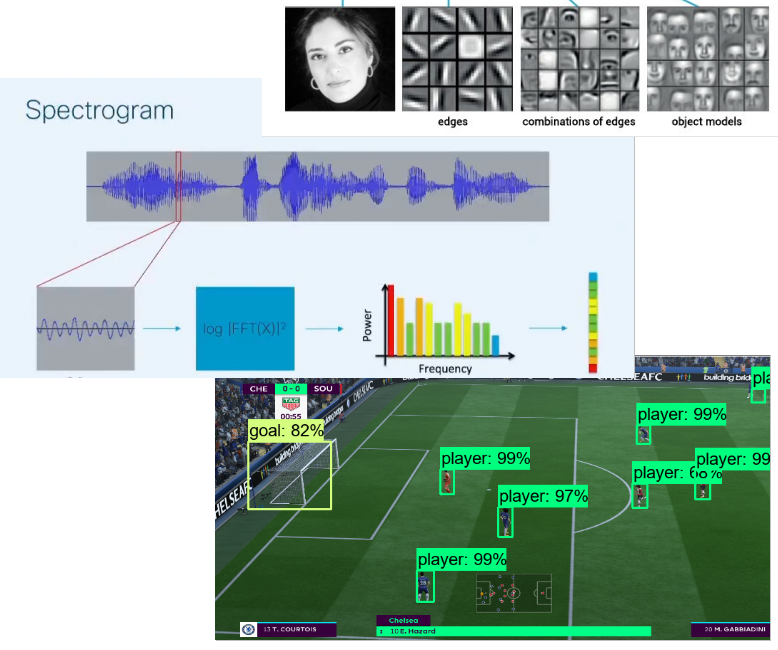
\includegraphics[width=0.9\textwidth]{example}
        \end{columns}
       
\end{frame}
%-


%*----------- SLIDE -------------------------------------------------------------
\begin{frame}[t]{Advantages to use Classical methods against to  Deep learning} 
        \begin{columns}[c]
                \column{.05\textwidth}
                \column{.6\textwidth}
                \newline
                \newline
                Works better with \textbf{small dataset}
                \newline
                \newline
                \textbf{Low} computional and financial cost
                \newline
                \newline
                The algorithms it's \textbf{easier} to understand and interpret
                \newline
                \newline
                \column{.35\textwidth}
        \end{columns}
       
\end{frame}
%*----------- SLIDE -------------------------------------------------------------
\begin{frame}[t]{Conclusion} 
    
\end{frame}
%-


    
    \begin{frame}[t, allowframebreaks]
        \frametitle{References}
        \bibliographystyle{amsalpha}
        \bibliography{biblio}
    \end{frame}

\end{document}